\section{Invariant Mass Distributions}
\label{sec:invmass}

Here the distribution of the invariant masses of the product particle of each
decay chain were plotted and examined.

\subsection{Two body $\psi(3770) \rightarrow D^0 \xbar{D^0}$ decay}
\label{sec:invmass/TwoBodyDecay}

The plot of the invariant mass distribution of the $D^0 \xbar{D^0}$, showing in
Figure \ref{fig:TwoBodyDecay}, matches exactly with the mass of the parent
$\psi(3770)$ particle\footnote{Mass of $\psi(3770) = 3773.15 \pm 0.33$
\MeV\cite{pdg}} , which is exactly as would be expected for a two body decay:

\begin{center}
    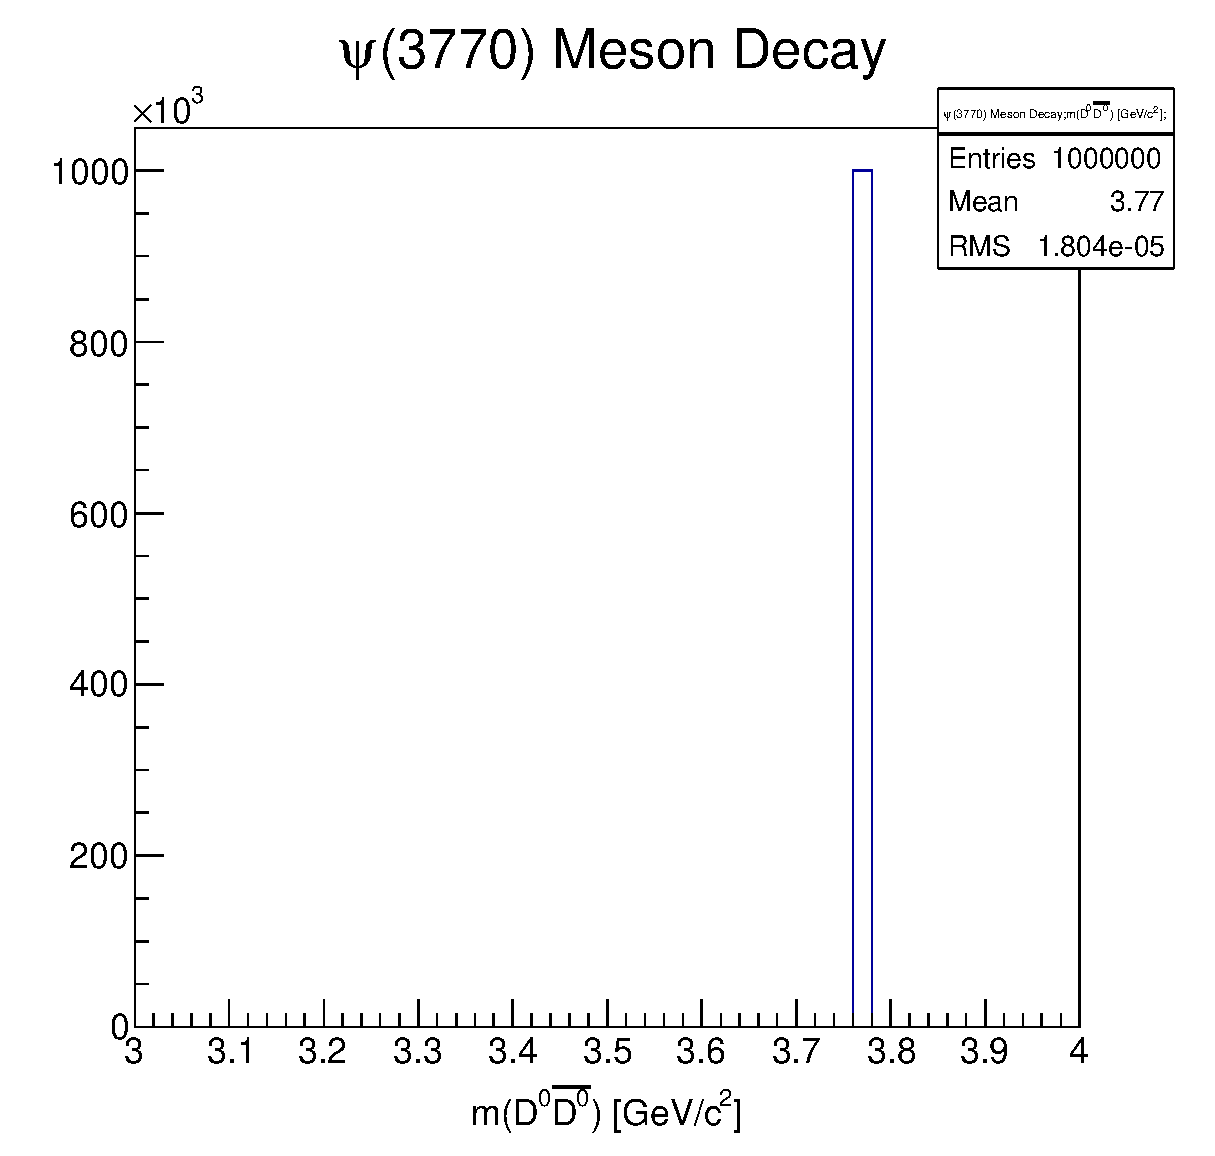
\includegraphics[width=\linewidth]{graphs/TwoBodyDecay}
    \captionof{figure}{The invariant mass distribution of the $D^0 \xbar{D^0}$
    corresponds exactly to the mass of the parent $\psi(3770)$.}
    \label{fig:TwoBodyDecay}
\end{center}

\subsection{Three body $B^+ \rightarrow D^0 \xbar{D^0} K^+$ decay}
\label{sec:invmass/ThreeBodyDecay}

For the three body decay, the invariant mass distributions produces a
3-dimensional plot of the invariant mass combinations. These weighted
distributions are shown below in Figures \ref{fig:ThreeBodyDecayDK_DK} and
\ref{fig:ThreeBodyDecayDK_DD}.

\begin{center}
    \includegraphics[width=\linewidth]{graphs/ThreeBodyDecayDK_DK}
    \captionof{figure}{3D plot showing the invariant mass distribution of $D^0
    K^+$ against $\xbar{D^0} K^+$. Note that the top of the distribution is roughly flat.}
    \label{fig:ThreeBodyDecayDK_DK}
\end{center}

\begin{center}
    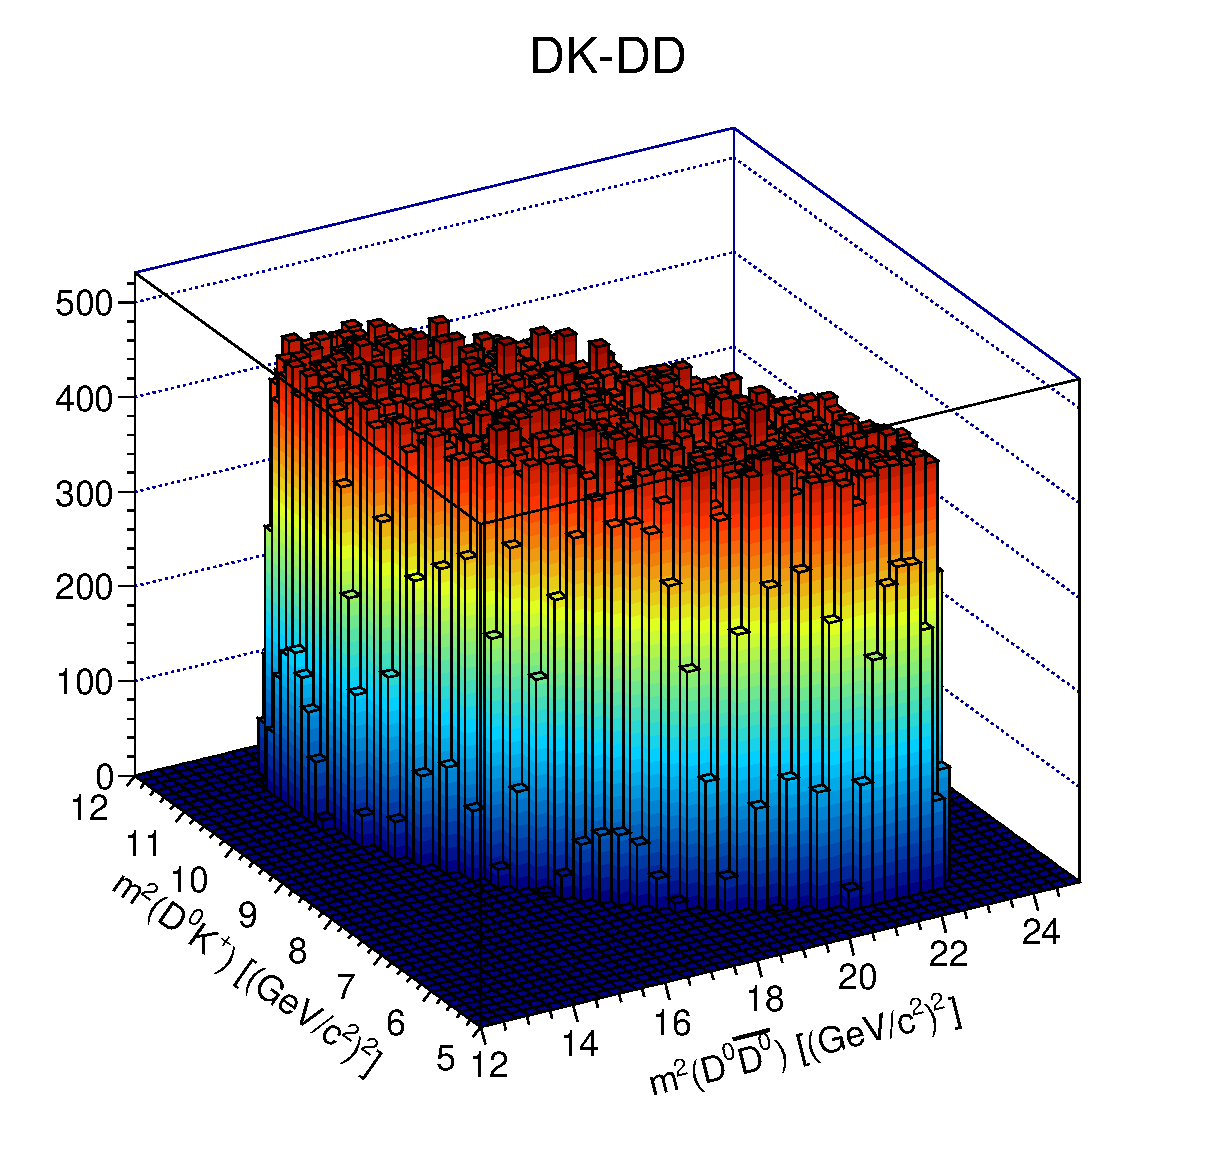
\includegraphics[width=\linewidth]{graphs/ThreeBodyDecayDK_DD}
    \captionof{figure}{3D plot showing the invariant mass distribution of $D^0
    K^+$ against $D^0 \xbar{D^0}$. Note that the top of this distribution is also roughly flat.}
    \label{fig:ThreeBodyDecayDK_DD}
\end{center}

Three body decay has a two-dimensional phase space, so these data are best
visualised as 3-dimensional density plots of the invariant mass distributions of
two of the three combinations of the particles. Note that all of the essential
information about the decay is contained in a single plot and the others can be
derived from the one plot due to momentum conservation laws.

This simulation does not take into account intermediate resonances, which have
the effect of altering the topology of the top of the plot so that it is no
longer roughly flat-topped. One such resonance, which will be discussed in
Section \ref{sec:decang-bdecay}, is of particular interest.

\subsection{Four body $D^0 \rightarrow K^+ K^- K^- \pi^+$ decay}
\label{sec:invmass/FourBodyDecay}

The four body decay produces a five dimensional phase space, which is projected
onto various axes so that they can be easily analysed and understood.

The following projected plots were produced:

\begin{center}
    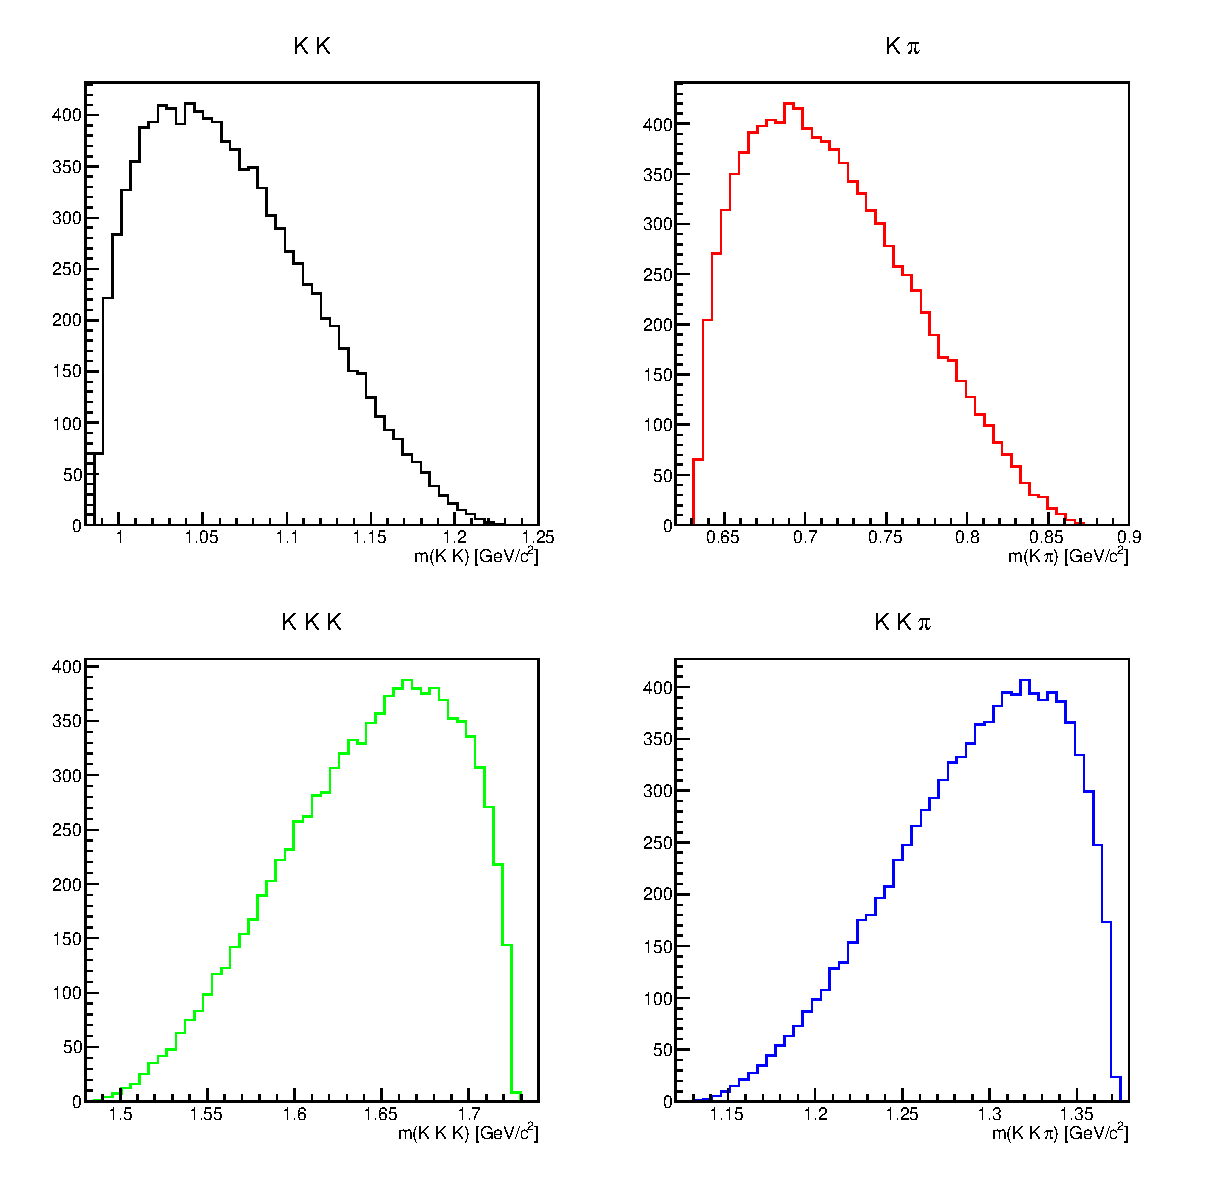
\includegraphics[width=\linewidth]{graphs/FourBodyDecay}
    \captionof{figure}{The projected plots of various invariant mass
    combinations for the four body decay $D^0 \rightarrow K^+ K^- K^- \pi^+$}
    \label{fig:FourBodyDecay}
\end{center}

Simulating intermediate resonances in this decay would produce rich strong phase
information arising from the interference between with the intermediate decays.
The possible intermediate resonances are tabulated below:

\end{multicols}

\newpage
{\centering
\begin{table}[H]
  \begin{tabu}{|[1.25pt] l |[1.25pt] p{2.5cm} |[1.25pt] p{3cm} |[1.25pt] l |[1.25pt] p{6cm} |[1.25pt]}
    \multicolumn{5}{c}{\Large{Light Unflavored Mesons} \large{($S=C=B=0$)}} \\
    \tabucline[1.25pt]{-}
    Particle Name & Mass [MeV] & Full width, $\Gamma$ [MeV] & $J^P$ & Decay
    Channel \\
    \tabucline[1.25pt]{-}
  
    $f_0(980)$ & 980 $\pm$ 10 & 40 $\rightarrow$ 100 & $0^+$ & 
      $f_0(980) \rightarrow K \xbar{K}$ 
    \\\hline
  
    $a_0(980)$ & 980 $\pm$ 20 & 50 $\rightarrow$ 100 & $0^+$ & 
      $a_0(980) \rightarrow K \xbar{K}$  
    \\\hline
  
    $\phi(1020)$ & 1019.45 $\pm$ 0.02 & 4.26 $\pm$ 0.04 & $1^-$ & 
      $\phi(1020) \rightarrow K^+K^-$  
    \\\hline
  
    $b_1(1235)$ & 1229.5 $\pm$ 3.2 & 142 $\pm$ 9 & $1^+$ &
      $b_1(1235) \rightarrow [\phi \rightarrow K^+ K^-] \pi$  \hfill and
      $b_1(1235) \rightarrow [K^*(892)^{\pm} \rightarrow K \pi]K^{\pm}$
    \\\hline
  
    $a_1(1260)$ & 1230 $\pm$ 40 & 250 $\rightarrow$ 600 & $1^+$ &
      $a_1(1260) \rightarrow [f_0(1370) \rightarrow K\xbar{K}]\pi$ \hfill and
      $a_1(1260) \rightarrow [f_2(1270) \rightarrow K\xbar{K}]\pi$ \hfill and
      $a_1(1260) \rightarrow K [\xbar{K}^*(892) \rightarrow K \pi] + c.c.$ 
    \\\hline
  
    $f_2(1270)$ & 1275.1 $\pm$ 1.2 & $185.1^{+2.9}_{-2.4}$ & $2+$ & 
      $f_2(1270) \rightarrow K\xbar{K}$
    \\\hline
  
    $f_1(1285)$ & 1281.8 $\pm$ 0.6 & 24.3 $\pm$ 1.1 & $1^+$ &
      $f_1(1285) \rightarrow K\xbar{K}\pi$
    \\\hline
  
    $\eta(1295)$ & 1294 $\pm$ 4 & 55 $\pm$ 5 & $0^-$ &
      $\eta(1295) \rightarrow a_0(980)\pi$
    \\\hline
  
    $a_2(1320)$ & 1318.3 $\pm$ 0.6 & 107 $\pm$ 5 & $2^+$ &
      $a_2(1320) \rightarrow K \xbar{K}$ 
    \\\hline
  
    $f_0(1370)$ & 1200 $\to$ 1500 & 200 $\to$ 500 & $0^+$ &
      $f_0(1370) \rightarrow K\xbar{K}$ 
    \\\hline
  
    $\eta(1405)$ & 1409.8 $\pm$ 2.5 & 51.1 $\pm$ 3.4 & $0^-$ &
      $\eta(1405) \rightarrow [a_0(980) \rightarrow K \xbar{K}] \pi$ \hfill and
      $\eta(1405) \rightarrow K \xbar{K} \pi$ \hfill and
      $\eta(1405) \rightarrow [K^*(892) \rightarrow K \pi] K$
    \\\hline
  
    $f_1(1420)$ & 1426.4 $\pm$ 0.9 & 54.9 $\pm$ 2.6 & $1^+$ & 
      $f_1(1420) \rightarrow K \xbar{K} \pi$ \hfill and
      $f_1(1420) \rightarrow K [\xbar{K}^*(892) \rightarrow K \pi] + c.c.$
    \\\hline
  
    $a_0(1450)$ & 1474 $\pm$ 19 & 265 $\pm$ 13 & $0^+$ & 
      $a_0(1450) \rightarrow K \xbar{K}$ 
    \\\hline
  
    $\rho(1450)$ & 1465 $\pm$ 13 & 265 $\pm$ 13 & $0^+$ & 
      $\rho(1450) \rightarrow K [\xbar{K}^*(892) \rightarrow K \pi] + c.c.$
      %(Possibly seen.)
    \\\hline
  
    $\eta(1475)$ & 1476 $\pm$ 4 & 85 $\pm$ 9 & $0^-$ &
      $\eta(1475) \rightarrow K \xbar{K} \pi$  \hfill and
      $\eta(1475) \rightarrow [a_0(980) \rightarrow K \xbar{K}] \pi$ \hfill and 
      $\eta(1475) \rightarrow K [\xbar{K}^*(892) \rightarrow K \pi] + c.c.$
    \\\hline
  
    $f_0(1500)$ & 1505 $\pm$ 6 & 109 $\pm$ 7 & $0^+$ &
      $f_0(1500) \rightarrow K \xbar{K}$
    \\\hline
  
    $f^{\prime}_2(1525)$ & 1525 $\pm$ 5 & $73^{+6}_{-5}$ & $2^+$ &
      $f^{\prime}_2(1525) \rightarrow K \xbar{K}$
    \\\hline
  
    $\eta_2(1645)$ & 1617 $\pm$ 5 & 181 $\pm$ 11 & $2^-$ &
      $\eta_2(1645) \rightarrow [a_2(1320) \rightarrow K \xbar{K}] \pi$ \hfill and
      $\eta_2(1645) \rightarrow K \xbar{K} \pi$ \hfill and
      $\eta_2(1645) \rightarrow [K^*(892) \rightarrow K \pi] \xbar{K}$ \hfill and
      $\eta_2(1645) \rightarrow [a_0(980) \rightarrow K \xbar{K}] \pi$
    \\\hline
  
    $\pi_2(1670)$ & 1672.2 $\pm$ 3.0 & 260 $\pm$ 9 & $2^-$ &
      $\pi_2(1670) \rightarrow [f_2(1270) \rightarrow K \xbar{K}] \pi$ \hfill and
      $\pi_2(1670) \rightarrow K [\xbar{K}^*(892) \rightarrow K \pi] + c.c.$
    \\\hline
  
    $\phi(1680)$ & 1680 $\pm$ 20 & 150 $\pm$ 50 & $1^-$ &
      $\phi(1680) \rightarrow K \xbar{K}$ \hfill and
      $\phi(1680) \rightarrow K [\xbar{K}^*(892) \rightarrow K \pi] + c.c.$
    \\\hline
  
    $\rho_3(1690)$ & 1688.8 $\pm$ 2.1 & 161 $\pm$ 10 & $3^-$ &
      $\rho_3(1690) \rightarrow K \xbar{K} \pi$ \hfill and
      $\rho_3(1690) \rightarrow K \xbar{K}$ \hfill and
      $\rho_3(1690) \rightarrow [a_2(1320) \rightarrow K \xbar{K}] \pi$
    \\\hline
  
    $\rho(1700)$ & 1720 $\pm$ 20 \newline ($\eta\rho^0$ \& $\pi^+\pi^-$) 
    %\footnote{$\eta\rho^0$ and $\pi^+\pi^-$ modes}
    %\addtocounter{footnote}{-1} \addtocounter{Hfootnote}{-1}
    %& 250 $\pm$ 100 \footnotemark{} & $1^-$ &
    & 250 $\pm$ 100 \newline ($\eta\rho^0$ \& $\pi^+\pi^-$) & $1^-$ &
      $\rho(1700) \rightarrow K \xbar{K}$ \hfill and
      $\rho(1700) \rightarrow K [\xbar{K}^*(892) \rightarrow K \pi] + c.c.$
    \\\hline
  
    $f_0(1710)$ & 1720 $\pm$ 6 & 135 $\pm$ 8 & $0^+$ &
      $f_0(1710) \rightarrow K \xbar{K}$
    \\\hline
  
    $\pi(1800)$ & 1812 $\pm$ 12 & 208 $\pm$ 12 & $0^-$ &
      $\pi(1800) \rightarrow [K^*(892) \rightarrow K \pi] K^-$
    \\\hline
  
    $\phi_3(1850)$ & 1854 $\pm$ 7 & $87^{+28}_{-23}$ & $3^-$ &
      $\phi_3(1850) \rightarrow K \xbar{K}$ \hfill and
      $\phi_3(1850) \rightarrow K [\xbar{K}^*(892) \rightarrow K \pi] + c.c.$
    \\\hline
  
    $f_2(1950)$ & 1944 $\pm$ 12 & 472 $\pm$ 18 & $2^+$ &
      $f_2(1950) \rightarrow K \xbar{K}$
    \\\hline
  
    $f_2(2010)$ & $2011^{+60}_{-80}$ & 202 $\pm$ 60 & $2^+$ &
      $f_2(2010) \rightarrow K \xbar{K}$
    \\\hline
  
    $a_4(2040)$ & $1996^{+10}_{-9}$ & $255^{+28}_{-24}$ & $4^+$ &
      $a_4(2040) \rightarrow K \xbar{K}$ \hfill and
      $a_4(2040) \rightarrow [f_2(1270) \rightarrow K \xbar{K}] \pi$
    \\\hline
  
    $f_4(2050)$ & 2018 $\pm$ 11 & 237 $\pm$ 18 & $4^+$ & 
      $f_4(2050) \rightarrow K \xbar{K}$ \hfill and
      $f_4(2050) \rightarrow [a_2(1320) \rightarrow K \xbar{K}] \pi$
    \\\hline
  
    $f_2(2300)$ & 2297 $\pm$ 28 & 149 $\pm$ 40 & $2^+$ &
      $f_2(2300) \rightarrow K \xbar{K}$
    \\
  
    \tabucline[1.25pt]{-}
  \end{tabu}
  \captionof{table}{Table of possible resonances for the light unflavored mesons.}
  \label{tab:LightUnflavoredMesons}
\end{table}
}


\newpage
{\centering
\begin{table}[H]
  \begin{tabu}{|[1.25pt] l |[1.25pt] l |[1.25pt] l |[1.25pt] l |[1.25pt] p{6cm} |[1.25pt]}
    \multicolumn{5}{c}{\Large{Strange Mesons} \large{($S=\pm1, C=B=0$)}} \\
    \tabucline[1.25pt]{-}
    Particle Name & Mass [MeV] & Full width, $\Gamma$ [MeV] & $J^P$ & Decay
    Channel \\
    \tabucline[1.25pt]{-}
  
    $K^*(892)$ & 895.5 $\pm$ 0.8 & 46.2 $\pm$ 1.3 & $1^-$ &
      \multirow{3}{*}{$K^*(892) \rightarrow K \pi$}
    \\\cline{1-4}
  
    $K^*(892)^{\pm}$ & 891.66 $\pm$ 0.26 & 50.8 $\pm$ 0.9 & $1^-$ &
    \\\cline{1-4}
  
    $K^*(892)^0$ & 895.94 $\pm$ 0.22 & 48.7 $\pm$ 0.8 & $1^-$ &
    \\\hline
  
    $K_1(1270)$ & 1272 $\pm$ 7 & 90 $\pm$ 20 & $1^+$ &
      $K_1(1270) \rightarrow K [f_0(1370) \rightarrow K \xbar{K}]$
    \\\hline
  
    $K_1(1400)$ & 1403 $ \pm$ 7 & 174 $\pm$ 13 & $1^+$ &
      $K_1(1400) \rightarrow K [f_0(1370) \rightarrow K \xbar{K}]$
    \\\hline
  
    $K^*(1410)$ & 1414 $\pm$ 15 & 232 $\pm$ 21 & $1^-$ &
      $K^*(1410) \rightarrow K \pi$
    \\\hline
  
    $K^*_0(1430)$ & 1425 $\pm$ 50 & 270 $\pm$ 80 & $0^+$ &
      $K^*_0(1430) \rightarrow K \pi$
    \\\hline
  
    $K^*_2(1430)^{\pm}$ & 1425.6 $\pm$ 1.5 & 98.5 $\pm$ 2.7 & $2^+$ &
      \multirow{2}{*}{$K^*_2(1430) \rightarrow K \pi$}
    \\\cline{1-4}
  
    $K^*_2(1430)^0$ & 1432.4 $\pm$ 1.3 & 109 $\pm$ 5 & $2^+$ &
    \\\hline
  
    $K^*(1680)$ & 1717 $\pm$ 27 & 322 $\pm$ 110 & $1^-$ & 
      $K^*(1680) \rightarrow K \pi$
    \\\hline
  
    $K_2(1770)$ & 1773 $\pm$ 8 & 186 $\pm$ 14 & $2^-$ &
      $ K_2(1770) \rightarrow K [f_2(1270 \rightarrow K \xbar{K}] $ \hfill and
      $ K_2(1770) \rightarrow K [\phi \rightarrow K^+ K^-]$
    \\\hline
  
    $K^*_3(1780)$ & 1776 $\pm$ 7 & 159 $\pm$ 21 & $3^-$ &
      $ K^*_3(1780) \rightarrow K \pi $
    \\\hline
  
    $K_2(1820)$ & 1816 $\pm$ 13 & 276 $\pm$ 35 & $2^-$ &
      $ K_2(1820) \rightarrow K [f_2(1270) \rightarrow K \xbar{K}] $
    \\\hline
  
    $K^*_4(2045)$ & 1045 $\pm$ 9 & 198 $\pm$ 30 & $4^+$ &
      $ K^*_4(2045) \rightarrow K \pi $
    \\
  
    \tabucline[1.25pt]{-}
  \end{tabu}
  \captionof{table}{Table of possible resonances for the strange mesons.}
  \label{tab:StrangeMesons}
\end{table}
}


\begin{multicols}{2}
